\documentclass[tikz,12pt]{standalone}
\usetikzlibrary{calc,intersections,through}
\begin{document}
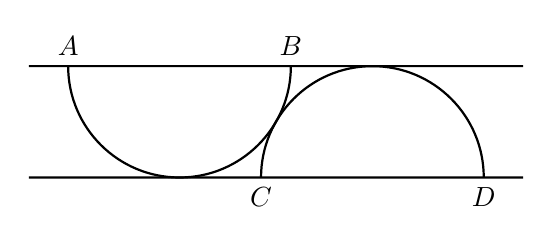
\begin{tikzpicture}[thick]
%DO NOT REMOVE THE SPACE BEFORE CLOSING PARENTHESES
\coordinate (A) at (0,{sqrt(2)} );
\path[name path=mid] (-.5,{sqrt(2)/2} )--(5,{sqrt(2)/2} );
\draw[name path=arcAB] (A) node[above] {$A$} arc (180:360:{sqrt(2)} ) node[above] {$B$};
\path[name intersections={of= arcAB and mid,by={X,Y}}];
\path[name path=arcY] (Y) arc (150:181:{sqrt(2)} );
\path[name path=bottom] (-.5,0)--(5,0);
\path[name intersections={of= arcY and bottom,by={C}}];
\draw (C) node[below] {$C$} arc (180:0:{sqrt(2)} ) node[below] {$D$};
\draw (-.5,0)--(C)--+({2*sqrt(2)+.5},0);
\draw (C) +({2*sqrt(2)+.5},{sqrt(2)} )--(-.5,{sqrt(2)} );
\end{tikzpicture}
\end{document}
